\documentclass[a4paper,11pt]{article} 

% ----------------
% SETTINGS
% ----------------
\usepackage[usenames,dvipsnames]{xcolor}
\usepackage{array}
\usepackage{caption}
\usepackage{colortbl}
\usepackage{float}
\usepackage{graphicx}
\usepackage{import}
\usepackage{listings}
\usepackage{tabularx}
\usepackage{tcolorbox}
\usepackage{url}
\usepackage{soul}
\usepackage{etoolbox} % if conditionals
\usepackage[outdir=./]{epstopdf}

\graphicspath{{figures/}{../figures/}}
\newcommand*{\CommonPath}{subfiles/}% 

% ----------------
% DOCUMENT
% ----------------
\begin{document}
% ----------------
% TITLE
% ----------------
\begin{titlepage}
\begin{center}
\textsc{\LARGE Integration Test Plan Document}\\[1.5cm] % 

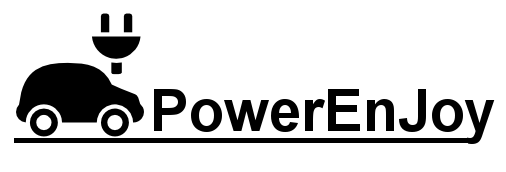
\includegraphics[width=10cm]{PowerEnJoy.png}\\
%\rule{\linewidth}{0.5mm} \\[0.7cm]
%{\huge \bfseries PowerEnJoy}\\[0.4cm] % Thesis title
%\rule{\linewidth}{0.5mm} \\[1.5cm]
 
\vfill
\vfill
\textbf{Authors:}\\
Patrizia Porati, Tommaso Sardelli\\[2.0cm] 


\vfill
\vfill

\includegraphics[width=50mm]{polimi.png}\\
%\textsc{Politecnico Di Milano}
\end{center}
\end{titlepage}

% ----------------
% TABLE OF CONTENTS
% ----------------
\tableofcontents
\pagebreak

% ----------------
% INTRODUCTION
% ----------------

\subimport{\CommonPath}{introduction.tex}

% ----------------
% INTEGRATION STRATEGY
% ----------------
\subimport{\CommonPath}{strategy.tex}

% Sequence of component / function integration
%\subimport{\CommonPath}{sequencecomponent.tex}

% ----------------
% INDIVIDUAL STEPS AND TEST DESCRIPTION
% ----------------
\subimport{\CommonPath}{description.tex}

% ----------------
% TOOLS AND TEST EQUIPMENT REQUIRED
% ----------------
%\subimport{\CommonPath}{tools.tex}

% ----------------
% PROGRAM STUBS AND TEST DATA REQUIRED
% ----------------
%\subimport{\CommonPath}{testdata.tex}

% ----------------
% EFFORT SPENT
% ----------------
\subimport{\CommonPath}{effort.tex}


\end{document}